\documentclass{scrartcl}
\usepackage[a4paper,left=1in,right=1in,top=1.2in,bottom=1in]{geometry}
\usepackage{siunitx}
\usepackage{graphicx}
\setkomafont{disposition}{\normalfont\bfseries}

%title
\title{Exercise 07:\\Conditional probability and signal-detection theory}
\subtitle{Theoretical Neuroscience I}
\author{Maria del Cerro \and Johannes G\"atjen \and Lorena Morton}

%use these for structure/overview
\newcommand\Question{%
  \textbf{Question:}%
}
\newcommand\Answer{%
  \textbf{Answer:}%
}

\begin{document}
\maketitle

We are given a function, which returns noisy responses to a series of target stimuli A and non-target stimuli B of different strengths.

We observe the responses $x$ to stimuli of strength 2, 7 and 20 and compare the resulting probability density functions of $P(x|A)$ and $P(x|B)$, which are shown in Figure \ref{pdf}. Stronger stimuli elicit stronger responses and B stimuli elicit lower average responses than A stimuli of equal strength. For all three stimulus strengths there is considerable overlap in the probability density functions, meaning it is not possible to perfectly distinguish between the stimulus types based on the response. Of the three stimulus strengths, 7 achieves the best separation of response strength between the stimulus types.

Figure \ref{conditional} shows the conditional likelihoods $L(A|x)$ and $L(B|x)$ for stimulus strength equal to 20. From the plot we can infer multiple things:
\begin{enumerate}
\item Only for response rates below 5 or above 35 we can be (almost) certain what the stimulus type is.
\item The optimal decision criterion is between 18 and 19, where $L(A|x) = L(B|x) = 0.5$, i.e. the lines cross.
\item The comparatively low steepness of the lines mean that there is a large range of values of $x$ for which the neuron cannot make perfect inferences about the stimulus.
\end{enumerate}

\begin{figure}
\centering
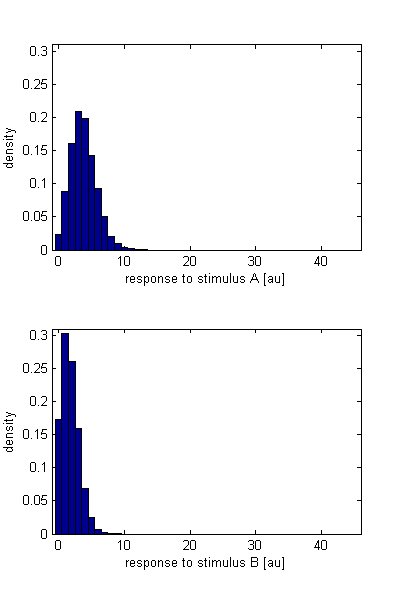
\includegraphics[trim = {0.1cm 0.6cm 0.9cm 1.1cm}, width=0.315\textwidth, clip]{../pics/dens2}
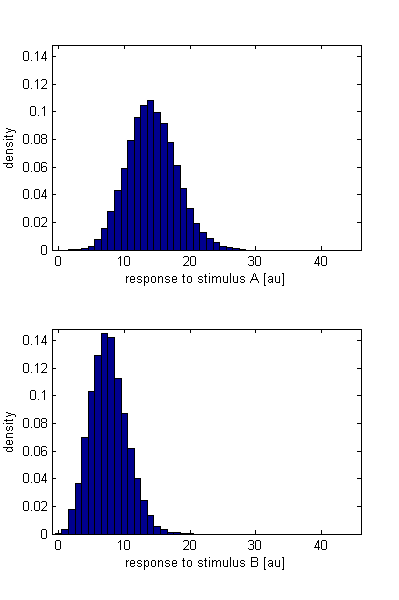
\includegraphics[trim = {0.1cm 0.6cm 0.9cm 1.1cm}, width=0.315\textwidth, clip]{../pics/dens7}
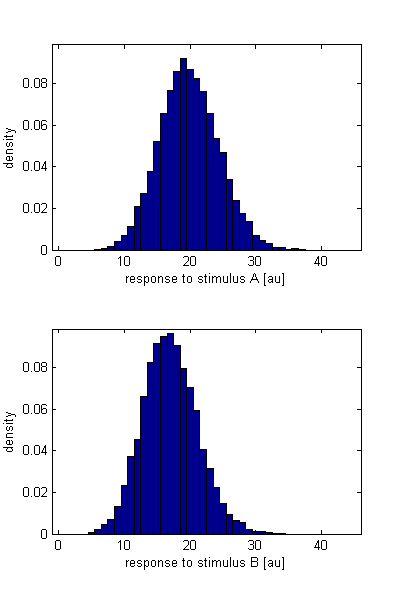
\includegraphics[trim = {0.1cm 0.6cm 0.9cm 1.1cm}, width=0.315\textwidth, clip]{../pics/dens20}
\caption{Columns left to right: Responses to stimuli of strength 2, 7 and 20. Top row: Responses to stimulus A. Bottom row: Responses to stimulus B. The probability density of the different response strengths is shown.}
\label{pdf}
\end{figure}

\begin{figure}
\centering
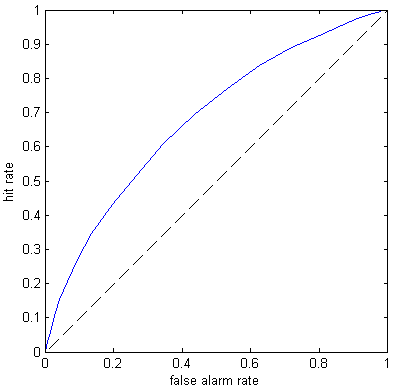
\includegraphics[width=0.6\textwidth]{../pics/roc}
\caption{The ROC curve for stimulus strength of 20. The hit rate (true positives, or correctly identified A stimuli) is plotted against the false alarm rate (false positives, or B stimuli incorrectly identified as A) in blue. Random guess is shown as a black dashed line. The area under the ROC curve is 0.681.}
\label{roc}
\end{figure}

\begin{figure}
\centering
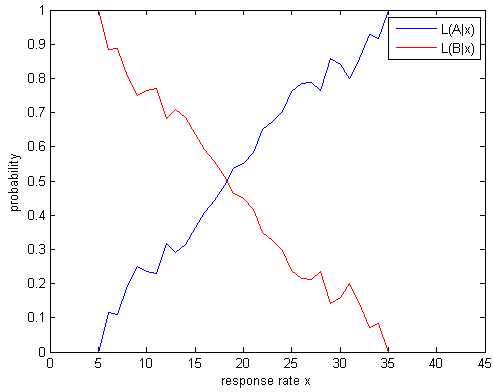
\includegraphics[width=0.6\textwidth]{../pics/conditional}
\caption{The likelihoods for A (blue) and B (red) under condition $x$ as a function of $x$ with stimulus strength 20, where $x$ is the response rate.}
\label{conditional}
\end{figure}

%include picture
%\begin{figure}
%\centering
%\includegraphics[trim = {1.3cm 0 2cm 0.9cm}, width=\textwidth, clip]{../pics/picname}
%\caption{caption text}
%\label{label}
%\end{figure}
\end{document}